% 定常迭代法：矩阵分裂、Richardson、Jacobi、Gauss--Seidel、SOR、SSOR与停止准则
\chapter{定常迭代法}
\label{sec:ls-stationary-iterations}
\label{chap:stationary-iterations}

设$\bm A\in\mathbb R^{d\times d}$可逆，要解$\bm A\bm x=\bm b$。第~\ref{chap:direct-linear-solvers}章的直接法先分解$\bm A$再回代，要存储并计算分解因子。矩阵很大而稀疏时，消元会在原来的零元位置产生大量非零元（填充），因子的存储和运算都可能难以承受。

本章换一条路线。选一个容易求解、又与$\bm A$相近的矩阵$\bm M$，每轮根据当前残差，解一个以$\bm M$为系数的方程得到修正量，再把修正量加到近似解上。每轮只需一次矩阵乘向量和一次简单求解（对角缩放或三角求解），不需要存储分解因子。这样做立即带来几个问题：这种更新从任意初值出发何时收敛到真解，收敛有多快，每轮要花多少计算，以及什么时候可以停下来。

回答收敛问题的工具来自第~\ref{chap:linear-recurrence-stability}章。那里证明了：仿射迭代$\bm x\mapsto\bm T\bm x+\bm c$从任意初值出发都收敛到同一个极限，当且仅当$\bm T$的谱半径小于一；渐近的收敛速度由谱半径决定，而非正规的$\bm T$在衰减之前还可能暂时放大误差。本章把每种方法都写成这种形式，收敛判断便归结为估计相应迭代矩阵的谱半径。三角求解采用第~\ref{sec:ls-lu}节的前代与回代。

第~\ref{sec:ls-matrix-splitting}节建立各方法共用的框架：由矩阵分裂得到不动点方程与修正形式，统一的执行流程，以及由谱半径给出的收敛判据。随后五节分别取不同的$\bm M$：Richardson迭代用标量矩阵，Jacobi迭代用$\bm A$的对角部分，Gauss--Seidel迭代用下三角部分，SOR在下三角修正中加入松弛参数，SSOR把前向与反向两次扫掠配成对称的一轮。此后每节先简述所取的$\bm M$与迭代形式，再分算法实现与算法分析两部分；算法实现逐步写出执行公式，并用同一个二维例子逐轮计算，便于对照各方法读取数据的方式。

SSOR的修正矩阵对称正定，这使它还能作为第~\ref{chap:krylov-methods}章共轭梯度法的预条件。最后一节讨论停止准则：达到残差要求与只是停止计算是两回事。

记号沿用本部分的约定：精确解记作$\bm x_\star$，第$k$轮近似记作$\bm x_k$，残差$\bm r_k=\bm b-\bm A\bm x_k$，修正量$\bm\delta_k$，误差$\bm e_k=\bm x_k-\bm x_\star$；向量的第$i$个分量写作$(\bm x_k)_i$。

\section{定常迭代}
\label{sec:ls-matrix-splitting}

\subsection{算法思想}

定常迭代的思路可以概括为两步：先把难解的方程拆成“容易求解的部分”与“其余部分”，从而改写成不动点方程；再从任意初值出发，用同一个固定的映射反复更新。

\paragraph{矩阵分裂}
直接求解$\bm A\bm x=\bm b$相当于处理$\bm A^{-1}$，对一般的$d$阶矩阵要做约$d^3$量级的运算。

我们可以换一个思路：把$\bm A$拆成两部分，
\begin{equation}
 \bm A=\bm M-\bm N ,
 \label{eq:ls-stationary-splitting}
\end{equation}
其中$\bm M$可逆并且极易求解，例如对角矩阵或三角矩阵，$\bm N=\bm M-\bm A$是剩下的部分。这种拆法称为\term{矩阵分裂}（matrix splitting）。

代入原方程，得
\[
 (\bm M-\bm N)\bm x=\bm b,\qquad\text{即}\qquad \bm M\bm x=\bm N\bm x+\bm b .
\]
两边左乘$\bm M^{-1}$，方程化为
\begin{equation}
 \bm x=\bm T\bm x+\bm c
 \label{eq:ls-stationary-fixed-point}
\end{equation}
其中$
 \bm T=\bm M^{-1}\bm N=\bm I-\bm M^{-1}\bm A$，$\bm c=\bm M^{-1}\bm b$。
这是一个\term{不动点方程}（fixed-point equation）：$\bm x_\star$正是仿射映射$\bm x\mapsto\bm T\bm x+\bm c$的不动点。$\bm T$称为\term{迭代矩阵}（iteration matrix），$\bm c$是常向量。

\paragraph{迭代求解}
有了不动点方程，自然的做法是把右端算出的值作为下一个近似，得到递推
\begin{equation}
 \bm x_{k+1}=\bm T\bm x_k+\bm c .
 \label{eq:ls-stationary-iteration}
\end{equation}
若$\bm x_k$收敛，极限必然满足式~\eqref{eq:ls-stationary-fixed-point}，也就是原方程的解。

整个过程中$\bm T$和$\bm c$固定不变，每一轮都用同一套规则修正当前的解，所以这类方法称为\term{定常迭代}（stationary iteration）。第~\ref{chap:krylov-methods}章的Krylov子空间法则不同：每一轮的搜索方向和步长系数都要由当前残差重新计算，相当于每轮的更新规则都在变化。

\paragraph{修正的迭代求解}
式~\eqref{eq:ls-stationary-iteration}中的$\bm M^{-1}$只是理论表示，执行时不形成逆矩阵。把它乘回去，得
\[ 
  \bm M\bm x_{k+1}=\bm N\bm x_k+\bm b=\bm M\bm x_k+(\bm b-\bm A\bm x_k) .
\]
记残差$\bm r_k=\bm b-\bm A\bm x_k$，修正量$\bm\delta_k=\bm x_{k+1}-\bm x_k$，就得到等价的修正形式
\begin{equation}
 \bm M\bm\delta_k=\bm r_k,\qquad \bm x_{k+1}=\bm x_k+\bm\delta_k .
 \label{eq:ls-stationary-correction}
\end{equation}
每轮只需算一次残差，再解一个以$\bm M$为系数的方程。

这个形式也说明了$\bm M$的作用。式~\eqref{eq:ls-stationary-correction}用$\bm M$代替了$\bm A$，只解近似的修正方程。$\bm M$越接近$\bm A$，修正越准确，但求解也越接近原问题的难度；$\bm M$越简单，每轮越便宜，修正却越粗糙。所以$\bm M$同时决定单步成本与每轮消除误差的程度。“容易求解”只说明每轮算得下去，并不保证迭代收敛，收敛要另行判断。

\paragraph{执行过程} 按这一形式，整个算法的执行流程如下。

先算$\bm r_0=\bm b-\bm A\bm x_0$，取停止阈值$\tau=\mathrm{atol}+\mathrm{rtol}\lVert\bm b\rVert_2$。

每一轮依次做三件事：
\begin{enumerate}
 \item \textbf{停止检查。}若$\lVert\bm r_k\rVert_2\leq\tau$，以“达到容差”结束；若$k=K$，以“步数耗尽”结束；出现溢出或非数时以“数值异常”结束，残差长期几乎不降时可报告“停滞”。只有第一种表示达到了残差目标，第~\ref{sec:ls-stationary-stopping}节再解释。
 \item \textbf{求修正量。}按式~\eqref{eq:ls-stationary-correction}解$\bm M\bm\delta_k=\bm r_k$；这一步随$\bm M$的选取而不同，是后面各节的主要内容。
 \item \textbf{更新。}令$\bm x_{k+1}=\bm x_k+\bm\delta_k$，按原方程重算$\bm r_{k+1}=\bm b-\bm A\bm x_{k+1}$，再令$k\leftarrow k+1$回到停止检查。
\end{enumerate}

后面各方法都沿用这套流程，只替换求$\bm\delta_k$的一步。

后面各方法用同一个小例子对照。下面先取对角矩阵作$\bm M$，只为核对流程中每个量怎样得到。
\begin{example}[定常迭代的贯穿例]
\label{ex:ls-stationary-running-example}
取下面的系数矩阵与右端，初值为$\bm x_0=\bm 0$：
\[
\bm A=\begin{bmatrix}4&1\\1&3\end{bmatrix},\qquad
\bm b=\begin{bmatrix}1\\2\end{bmatrix}.
\]
精确解为$\bm x_\star=(1/11,7/11)^\top\approx(0.0909,0.6364)^\top$。

取$\bm M=\operatorname{diag}(4,3)$，解修正方程只需逐分量相除。第一轮从$\bm r_0=\bm b$出发，修正量与新的近似解为
\[
 \bm\delta_0=\begin{bmatrix}\tfrac14\\\tfrac23\end{bmatrix},\qquad
 \bm x_1=\begin{bmatrix}\tfrac14\\\tfrac23\end{bmatrix},
\]
按原方程算出的残差为
\[
 \bm r_1=\bm b-\bm A\bm x_1=\begin{bmatrix}-\tfrac23\\-\tfrac14\end{bmatrix}.
\]
第二轮同样先求修正量并更新：
\[
 \bm\delta_1=\begin{bmatrix}-\tfrac16\\-\tfrac1{12}\end{bmatrix},\qquad
 \bm x_2=\begin{bmatrix}\tfrac1{12}\\\tfrac7{12}\end{bmatrix},
\]
再算出残差
\[
 \bm r_2=\begin{bmatrix}\tfrac1{12}\\\tfrac16\end{bmatrix}.
\]
残差范数依次约为$2.24$、$0.71$、$0.19$，在下降但没有降到零。每轮的修正方程都精确地解出了，$\bm x_2$却仍不是解，因为修正方程用$\bm M$代替了$\bm A$；是否解完，只能由原方程的残差判断。
\end{example}

\paragraph{按元素构造分裂}
后面的方法要按元素构造$\bm M$，为此统一写
\begin{equation}
\bm A=\bm D+\bm L+\bm U ,
 \label{eq:ls-stationary-dlu-splitting}
\end{equation}
其中$\bm D$是$\bm A$的对角部分，$\bm L$与$\bm U$分别是严格下三角与严格上三角部分，元素保留$\bm A$中原来的符号。

\subsection{算法分析}

精确解满足$\bm x_\star=\bm T\bm x_\star+\bm c$，与式~\eqref{eq:ls-stationary-iteration}相减，误差$\bm e_k=\bm x_k-\bm x_\star$满足
\[
 \bm e_{k+1}=\bm T\bm e_k=(\bm I-\bm M^{-1}\bm A)\bm e_k .
\]
每轮误差乘同一个固定矩阵，这正是第~\ref{chap:linear-recurrence-stability}章研究过的矩阵幂问题，下面据此给出收敛判据。

\paragraph{收敛条件}
各方法是否收敛，取决于迭代矩阵$\bm T=\bm I-\bm M^{-1}\bm A$每轮把误差变成什么。下面的定理把收敛问题归结为$\bm T$的谱半径，后面各节只需分别估计各自的$\rho(\bm T)$。
\begin{theorem}[定常迭代的收敛判据]
\label{thm:ls-stationary-convergence}
设$\bm A$与$\bm M$可逆，$\bm x_\star$是$\bm A\bm x=\bm b$的解。按$\bm M\bm\delta_k=\bm r_k$，$\bm x_{k+1}=\bm x_k+\bm\delta_k$迭代时，误差满足
\begin{equation}
\bm e_{k+1}=\bm T\bm e_k,\qquad \bm e_k=\bm T^k\bm e_0 ,
 \label{eq:ls-stationary-error-recursion}
\end{equation}
且迭代对任意初值$\bm x_0$都收敛到$\bm x_\star$，当且仅当$\rho(\bm T)<1$。
\end{theorem}
\begin{proof}
由$\bm r_k=\bm b-\bm A\bm x_k=-\bm A\bm e_k$，更新式给出
\[
 \bm e_{k+1}=\bm e_k-\bm M^{-1}\bm A\bm e_k=\bm T\bm e_k ,
\]
归纳得$\bm e_k=\bm T^k\bm e_0$。

更新也可写成仿射映射$\bm x\mapsto\bm T\bm x+\bm M^{-1}\bm b$。因为$\bm I-\bm T=\bm M^{-1}\bm A$可逆，它只有一个固定点，满足$\bm M^{-1}\bm A\bm x=\bm M^{-1}\bm b$，就是$\bm x_\star$。

由第~\ref{sec:ls-convergence}章的定理~\ref{thm:ls-affine-common-limit}，从任意初值出发的轨迹都收敛到同一个向量当且仅当$\rho(\bm T)<1$，而这个共同极限只能是固定点$\bm x_\star$。
\end{proof}

算法可执行与算法收敛是两个条件：$a_{i,i}\neq0$只保证每轮能算下去，不保证$\rho(\bm T)<1$；反过来，$\rho(\bm T)<1$也不保证某种逐元素公式可以执行。

\paragraph{收敛速度与总成本}
渐近速度由$\bm T$的谱控制：由定理~\ref{thm:ls-gelfand-formula}，$\lVert\bm T^k\rVert^{1/k}\to\rho(\bm T)$，误差每缩小十倍约需$1/\log_{10}(1/\rho(\bm T))$轮。非正规的$\bm T$还可能在衰减前暂时放大误差（第~\ref{sec:ls-convergence-rate-transient}节），所以前几轮的表现不能代替渐近判断。

收缩率与单步成本是两件事。达到给定精度的总工作量约为所需轮数乘每轮成本；每轮成本包括一次求$\bm\delta_k$和一次计算残差的矩阵乘向量。$\bm M$越接近$\bm A$，谱半径通常越小，但求解$\bm M$越贵。比较不同分裂时要把两者合起来看，不能只比较谱半径或只比较单步成本。

\section{Richardson迭代}
\label{sec:ls-richardson}

最简单的选择是用标量矩阵代替$\bm A$：取非零步长$\alpha$，令修正矩阵$\bm M=\alpha^{-1}\bm I$。这相当于认为$\bm A$在各个方向上都大致把向量放大$1/\alpha$倍。迭代矩阵为$\bm T=\bm I-\alpha\bm A$，常向量为$\bm c=\alpha\bm b$。

$\bm M$是单位矩阵的倍数，修正方程$\alpha^{-1}\bm\delta_k=\bm r_k$两边乘以$\alpha$就解出了修正量：
\begin{equation}
 \bm\delta_k=\alpha\bm r_k ,\qquad\text{即}\qquad (\bm\delta_k)_i=\alpha(\bm r_k)_i .
 \label{eq:ls-richardson-correction}
\end{equation}
每个残差分量按同一比例转成对应分量的修正，不需要读取$\bm A$的任何元素。

把修正量加到当前近似上，一轮迭代就是
\begin{equation}
 \bm x_{k+1}=\bm x_k+\alpha(\bm b-\bm A\bm x_k)=(\bm I-\alpha\bm A)\bm x_k+\alpha\bm b .
 \label{eq:ls-richardson-update}
\end{equation}

\subsection{算法实现}

输入是$\bm A$与$\bm b$，输出是近似解$\bm x$。除第~\ref{sec:ls-matrix-splitting}节执行流程中的初值、容差与最大轮数外，还要预先选定步长$\alpha$。下面在例~\ref{ex:ls-stationary-running-example}上取$\alpha=1/4$，每一步之后给出前两轮的数值。
\begin{enumerate}
 \item \textbf{核对步长。}使用对称正定情形的收敛保证（定理~\ref{thm:ls-richardson-spd}）时，先按已知的谱界核对
 \begin{equation}
  0<\alpha<\frac{2}{\lambda_{\max}} ;
  \label{eq:ls-richardson-step-range}
 \end{equation}
 
 例中$\bm A$对称正定，最大特征值为$(7+\sqrt5)/2\approx4.618<5$，所以$2/\lambda_{\max}>2/5>1/4$，步长$\alpha=1/4$在收敛区间内。

 \item \textbf{求修正量。}通过停止检查后，按式~\eqref{eq:ls-richardson-correction}把残差的每个分量乘以同一个步长：
 \[
  (\bm\delta_k)_i=\alpha(\bm r_k)_i,\qquad i=1,\ldots,d .
 \]

 例中第一轮的残差为$\bm r_0=\bm b-\bm A\bm 0=(1,2)^\top$，于是
 \[
  \bm\delta_0=\frac14\begin{bmatrix}1\\2\end{bmatrix}=\begin{bmatrix}\tfrac14\\\tfrac12\end{bmatrix}.
 \]

 \item \textbf{更新并重算残差。}令$\bm x_{k+1}=\bm x_k+\bm\delta_k$，再用原矩阵算一次$\bm q_{k+1}=\bm A\bm x_{k+1}$，得到残差$\bm r_{k+1}=\bm b-\bm q_{k+1}$。按分量写出就是
 \begin{equation}
  (\bm r_{k+1})_i=b_i-\sum_{j=1}^d a_{i,j}(\bm x_{k+1})_j ,\qquad i=1,\ldots,d .
  \label{eq:ls-stationary-residual-update}
 \end{equation}
 重算的残差既用于下一轮的停止检查，也是下一轮修正的输入，所以每轮只需一次矩阵乘向量。

 例中$\bm x_1=\bm 0+\bm\delta_0=(1/4,1/2)^\top$，
 \[
  \begin{aligned}
  (\bm r_1)_1&=1-\bigl(4\cdot\tfrac14+1\cdot\tfrac12\bigr)=1-\tfrac32=-\tfrac12,\\
  (\bm r_1)_2&=2-\bigl(1\cdot\tfrac14+3\cdot\tfrac12\bigr)=2-\tfrac74=\tfrac14 .
  \end{aligned}
 \]

 \item \textbf{进入下一轮。}令$k\leftarrow k+1$，回到执行流程的停止检查；没有停止时重复第2、3步。

 例中$\lVert\bm r_1\rVert_2\approx0.56$，继续第二轮。修正量与新的近似解为
 \[
  \bm\delta_1=\frac14\bm r_1=\begin{bmatrix}-\tfrac18\\\tfrac1{16}\end{bmatrix},\qquad
  \bm x_2=\bm x_1+\bm\delta_1=\begin{bmatrix}\tfrac18\\\tfrac9{16}\end{bmatrix}.
 \]

\end{enumerate}

两轮后残差长度约为$0.198$。与精确解比较，误差为
\[
\bm e_2=\bm x_2-\bm x_\star=\begin{bmatrix}\tfrac3{88}\\-\tfrac{13}{176}\end{bmatrix},
\]
长度约$0.081$。由$\bm e_k=-\bm A^{-1}\bm r_k$，误差是残差经$\bm A^{-1}$变换后的结果，两者方向和大小都不同，是不同的数值对象。

\subsection{算法分析}

\paragraph{收敛条件与最优步长}
当$\bm A$实对称正定时，误差递推$\bm e_{k+1}=(\bm I-\alpha\bm A)\bm e_k$可以按特征方向分开看：把$\bm e_k$按$\bm A$的正交特征基展开，特征值$\lambda_i$对应的误差系数每轮乘$1-\alpha\lambda_i$。由定理~\ref{thm:ls-stationary-convergence}，收敛条件和最优步长都可以从这些倍率直接读出。
\begin{theorem}[对称正定矩阵的Richardson迭代]
\label{thm:ls-richardson-spd}
设$\bm A$实对称正定，特征值落在$[\lambda_{\min},\lambda_{\max}]$中且两端取到。Richardson迭代对所有初值收敛当且仅当$0<\alpha<2/\lambda_{\max}$；最优固定步长为$\alpha_\star=2/(\lambda_{\min}+\lambda_{\max})$，对应的收缩因子为
\begin{equation}
\rho(\bm T)=\frac{\kappa_2(\bm A)-1}{\kappa_2(\bm A)+1}.
 \label{eq:ls-richardson-optimal-rate}
\end{equation}
\end{theorem}
\begin{proof}
由上面的特征展开，
\[
 \rho(\bm T)=\max_i|1-\alpha\lambda_i| ,
\]
它小于一当且仅当每个$\alpha\lambda_i\in(0,2)$，即$0<\alpha<2/\lambda_{\max}$。

$|1-\alpha\lambda|$作为$\lambda$的函数在区间端点取最大，所以
\[
\rho(\bm T)=q(\alpha)=\max\{|1-\alpha\lambda_{\min}|,\ |1-\alpha\lambda_{\max}|\}.
\]
$\alpha$从零增大时，$|1-\alpha\lambda_{\min}|$先变小，$|1-\alpha\lambda_{\max}|$在$\alpha>1/\lambda_{\max}$后变大；两者大小相等、符号相反时最大值最小，即
\[
 1-\alpha\lambda_{\min}=\alpha\lambda_{\max}-1 ,
\]
解得$\alpha_\star$。代回得
\[
 q(\alpha_\star)=\frac{\lambda_{\max}-\lambda_{\min}}{\lambda_{\max}+\lambda_{\min}} ,
\]
再用$\kappa_2(\bm A)=\lambda_{\max}/\lambda_{\min}$即得式~\eqref{eq:ls-richardson-optimal-rate}。
\end{proof}
步长过大时，大特征值方向的倍率$1-\alpha\lambda_{\max}$小于$-1$，误差在该方向上正负交替地放大；所以残差没有消失并不意味着应当加大修正。

一般非对称矩阵仍可使用同一更新式，但特征值可能是复数，也没有正交特征基，上面的步长区间与最优步长不再直接适用；这时要回到定理~\ref{thm:ls-stationary-convergence}，检查$\rho(\bm I-\alpha\bm A)<1$。

\paragraph{收敛速度与代价}
谱范围越宽，$\kappa_2(\bm A)$越大，收缩因子越接近一，收敛越慢。实际中谱端点往往未知，步长按已知的谱界选取，例如用$\lVert\bm A\rVert$作$\lambda_{\max}$的上界。

贯穿例中$\lambda_{\min}\approx2.382$，$\lambda_{\max}\approx4.618$：$\alpha=1/4$时$\rho(\bm T)=1-\lambda_{\min}/4\approx0.40$；最优步长$\alpha_\star=2/7$给出$\rho(\bm T)=\sqrt5/7\approx0.32$。

每轮的主要代价是一次矩阵乘向量，约$2\operatorname{nnz}(\bm A)$次运算。停止时的残差与解误差之间的关系在第~\ref{sec:ls-stationary-stopping}节解释。

\section{Jacobi迭代}
\label{sec:ls-jacobi}

Richardson迭代对所有方程用同一个比例，没有利用各个方程自身的尺度。Jacobi迭代取$\bm A$的对角部分作修正矩阵，$\bm M=\bm D$：第$i$个方程只用来修正“自己的”未知量$x_i$，其余分量一律取上一轮的值。对角元相对非对角元越大，$\bm D$越接近$\bm A$，这个近似越好；例~\ref{ex:ls-stationary-running-example}所取的$\bm M=\operatorname{diag}(4,3)$正是这个分裂。

\paragraph{求修正量}
修正方程$\bm D\bm\delta_k=\bm r_k$的系数矩阵只有对角元，按元素写出是
\[
 \begin{bmatrix}a_{1,1}&&&\\&a_{2,2}&&\\&&\ddots&\\&&&a_{d,d}\end{bmatrix}
 \begin{bmatrix}(\bm\delta_k)_1\\(\bm\delta_k)_2\\\vdots\\(\bm\delta_k)_d\end{bmatrix}
 =\begin{bmatrix}(\bm r_k)_1\\(\bm r_k)_2\\\vdots\\(\bm r_k)_d\end{bmatrix},
\]
其中空白位置都是零。左边乘出来，第$i$行只剩对角元一项，所以按行的方程是
\[
 a_{i,i}(\bm\delta_k)_i=(\bm r_k)_i\qquad(i=1,\ldots,d).
\]
与前代不同，这里每个方程只含一个未知量，不需要用到其他方程的结果。两边除以$a_{i,i}$，得
\begin{equation}
 (\bm\delta_k)_i=\frac{(\bm r_k)_i}{a_{i,i}}\qquad(i=1,\ldots,d).
 \label{eq:ls-jacobi-correction}
\end{equation}
耦合的方程组就这样拆成了$d$个独立的标量计算，可以按任意次序或同时进行。

\paragraph{迭代公式}
把式~\eqref{eq:ls-jacobi-correction}加到当前近似上，得到第$i$个分量的新值
\begin{equation}
 (\bm x_{k+1})_i=(\bm x_k)_i+\frac{(\bm r_k)_i}{a_{i,i}}\qquad(i=1,\ldots,d),
 \label{eq:ls-jacobi-update}
\end{equation}
写成向量形式是
\[
  \bm x_{k+1}=\bm x_k+\bm D^{-1}\bm r_k .
\]

残差$\bm r_k$由上一轮的$\bm x_k$算出，所以各分量可以同时计算。

\subsection{算法实现}

输入是$\bm A$与$\bm b$，输出是近似解$\bm x$，执行流程的参数之外不需要其他参数。停止检查与残差重算沿用第~\ref{sec:ls-matrix-splitting}节的流程，求修正量的一步换成逐分量除以对角元。实现时维护新旧两个向量：旧向量$\bm x_k$在整轮中只读不写，新分量写进另一个向量。下面在例~\ref{ex:ls-stationary-running-example}上给出前两轮，并标明每个代入值的轮次。
\begin{enumerate}
 \item \textbf{检查对角元。}确认所有$a_{i,i}\neq0$，并保存倒数$1/a_{i,i}$。若某个对角元为零，当前的变量排列下方法不可执行；重排行列属于另一步，重排后要重新核对条件。

 例中$a_{1,1}=4$，$a_{2,2}=3$，都不为零。

 \item \textbf{逐分量计算新值。}根据式~\eqref{eq:ls-jacobi-update}，对$i=1,\ldots,d$计算$(\bm x_{k+1})_i$，其中的残差$\bm r_k$是由旧向量算出的。各分量只读旧向量和$\bm r_k$，彼此不依赖，可以按任意次序或并行计算。

 例中第一轮的残差为$\bm r_0=\bm b=(1,2)^\top$：
 \[
  \begin{aligned}
  (\bm x_1)_1&=(\bm x_0)_1+\frac{(\bm r_0)_1}{a_{1,1}}=0+\frac14=\frac14,\\
  (\bm x_1)_2&=(\bm x_0)_2+\frac{(\bm r_0)_2}{a_{2,2}}=0+\frac23=\frac23 .
  \end{aligned}
 \]

 \item \textbf{整体替换并重算残差。}全部$d$个分量算完之后，才用新向量替换旧向量，并按原方程重算
 \[
  (\bm r_{k+1})_i=b_i-\sum_{j=1}^d a_{i,j}(\bm x_{k+1})_j ,\qquad i=1,\ldots,d .
 \]
 若算出一个分量就覆盖旧值，再按新值重算后面的残差分量，后面的行就会读到本轮的新值，方法就不再是Jacobi迭代。单个分量变化很小，也不能代替这个全局残差检查。

 例中$\bm x_1=(1/4,2/3)^\top$，
 \[
  \begin{aligned}
  (\bm r_1)_1&=1-\bigl(4\cdot\tfrac14+1\cdot\tfrac23\bigr)=-\tfrac23,\\
  (\bm r_1)_2&=2-\bigl(1\cdot\tfrac14+3\cdot\tfrac23\bigr)=-\tfrac14 .
  \end{aligned}
 \]
 两个残差分量都变成负的，说明两个修正都过了头：每个分量都在假定另一个分量不变的前提下修正，而另一个分量同时也在变。

 \item \textbf{进入下一轮。}令$k\leftarrow k+1$，回到执行流程的停止检查；没有停止时重复第2、3步。

 例中$\lVert\bm r_1\rVert_2\approx0.71$，继续第二轮。用$\bm r_1=(-2/3,-1/4)^\top$修正$\bm x_1=(1/4,2/3)^\top$：
 \[
  \begin{aligned}
  (\bm x_2)_1&=(\bm x_1)_1+\frac{(\bm r_1)_1}{a_{1,1}}=\frac14-\frac{2/3}{4}=\frac1{12},\\
  (\bm x_2)_2&=(\bm x_1)_2+\frac{(\bm r_1)_2}{a_{2,2}}=\frac23-\frac{1/4}{3}=\frac7{12},
  \end{aligned}
 \]
 重算残差得
 \[
  \begin{aligned}
  (\bm r_2)_1&=1-\bigl(4\cdot\tfrac1{12}+1\cdot\tfrac7{12}\bigr)=\tfrac1{12},\\
  (\bm r_2)_2&=2-\bigl(1\cdot\tfrac1{12}+3\cdot\tfrac7{12}\bigr)=\tfrac16 .
  \end{aligned}
 \]
 结果与例~\ref{ex:ls-stationary-running-example}中按修正量计算的完全一致，残差长度由约$0.71$降到约$0.19$。
\end{enumerate}

\subsection{算法分析}

\paragraph{收敛条件}
Jacobi迭代矩阵$\bm T_{\mathrm J}=-\bm D^{-1}(\bm L+\bm U)$第$i$行的非对角元为$-a_{i,j}/a_{i,i}$，对角元为零。当每行的对角元压过同一行其余元素时，这个矩阵的行和范数小于一，由此得到常用的充分条件。

称$\bm A$\term{严格行对角占优}（strictly row diagonally dominant），如果每行都有$|a_{i,i}|>\sum_{j\neq i}|a_{i,j}|$。
\begin{theorem}[Jacobi迭代的收敛条件]
\label{thm:ls-jacobi-convergence}
若$\bm A$严格行对角占优，则
\begin{equation}
q=\lVert\bm T_{\mathrm J}\rVert_\infty=\max_i\frac{\sum_{j\neq i}|a_{i,j}|}{|a_{i,i}|}<1,
 \label{eq:ls-jacobi-contraction}
\end{equation}
Jacobi迭代对所有初值收敛，且$\lVert\bm e_k\rVert_\infty\leq q^k\lVert\bm e_0\rVert_\infty$。
\end{theorem}
\begin{proof}
$\infty$-范数诱导的矩阵范数等于最大行绝对值和，$\bm T_{\mathrm J}$第$i$行的绝对值和正是$\sum_{j\neq i}|a_{i,j}|/|a_{i,i}|$，对角占优使它小于一。由定理~\ref{thm:ls-stationary-convergence}，$\bm e_k=\bm T_{\mathrm J}^k\bm e_0$，再用范数的次乘性得$\lVert\bm e_k\rVert_\infty\leq q^k\lVert\bm e_0\rVert_\infty\to0$。
\end{proof}
贯穿例两行的比值分别为$1/4$与$1/3$，所以$q=1/3$。

对称正定本身并不够。$\bm A=\bm I+2\bm 1\bm 1^\top\in\mathbb R^{3\times3}$的特征值为$7,1,1$，是对称正定矩阵，而它的对角部分为$3\bm I$，于是
\[
 \bm T_{\mathrm J}=-\tfrac23(\bm 1\bm 1^\top-\bm I) .
\]
它沿$\bm 1$方向的特征值为$-\tfrac23(3-1)=-4/3$，在与$\bm 1$正交的方向上为$2/3$，所以$\rho(\bm T_{\mathrm J})=4/3$，迭代发散。

\paragraph{并行性}
各分量的更新互不依赖，可以并行；一轮工作量与$\operatorname{nnz}(\bm A)$同阶。单步便宜、易于并行，不等于误差衰减快：$\rho(\bm T_{\mathrm J})$接近一时需要很多轮。

\paragraph{数值敏感度}
式~\eqref{eq:ls-jacobi-correction}要除以对角元。很小的对角元会把残差分量放大成很大的修正，也放大其中的舍入误差。

\section{Gauss--Seidel迭代}
\label{sec:ls-gauss-seidel}

Jacobi迭代求第$i$个分量的修正时，只用本轮开始时的残差，没有计入本轮已经求出的前面各分量的修正。Gauss--Seidel迭代按顺序处理各行，把已经求出的修正立即计入后面的方程；原方程没有变，改变的只是读取信息的时刻。这相当于修正矩阵取$\bm A$的下三角部分，$\bm M=\bm D+\bm L$：它比$\bm D$多保留了严格下三角的元素，更接近$\bm A$，而下三角方程仍可以逐行前代求解。

\paragraph{求修正量}
修正方程$(\bm D+\bm L)\bm\delta_k=\bm r_k$按元素写出是
\[
 \begin{bmatrix}a_{1,1}&&&\\a_{2,1}&a_{2,2}&&\\\vdots&\vdots&\ddots&\\a_{d,1}&a_{d,2}&\cdots&a_{d,d}\end{bmatrix}
 \begin{bmatrix}(\bm\delta_k)_1\\(\bm\delta_k)_2\\\vdots\\(\bm\delta_k)_d\end{bmatrix}
 =\begin{bmatrix}(\bm r_k)_1\\(\bm r_k)_2\\\vdots\\(\bm r_k)_d\end{bmatrix},
\]
其中对角线以上的空白位置都是零。左边乘出来，第$i$行只含前$i$个分量，按行的方程是
\[
 \sum_{j<i}a_{i,j}(\bm\delta_k)_j+a_{i,i}(\bm\delta_k)_i=(\bm r_k)_i\qquad(i=1,\ldots,d).
\]
这是第~\ref{sec:ls-lu}节的下三角方程，按前代求解。第一个方程只含$(\bm\delta_k)_1$，得
\[
 (\bm\delta_k)_1=\frac{(\bm r_k)_1}{a_{1,1}} .
\]
第二个方程中$(\bm\delta_k)_1$已经求出，移项后得
\[
 (\bm\delta_k)_2=\frac{(\bm r_k)_2-a_{2,1}(\bm\delta_k)_1}{a_{2,2}} .
\]
一般地，第$i$个方程中$(\bm\delta_k)_1,\ldots,(\bm\delta_k)_{i-1}$已由前面的方程求出，把它们移到右边，再除以$a_{i,i}$，得
\begin{equation}
 (\bm\delta_k)_i=\frac{(\bm r_k)_i-\sum_{j<i}a_{i,j}(\bm\delta_k)_j}{a_{i,i}}\qquad(i=1,\ldots,d).
 \label{eq:ls-gauss-seidel-correction}
\end{equation}
与Jacobi的式~\eqref{eq:ls-jacobi-correction}相比，分子多减去了前面各分量的修正对第$i$个方程的影响。$(\bm r_k)_i-\sum_{j<i}a_{i,j}(\bm\delta_k)_j$正是前$i-1$个分量修正之后第$i$个方程的残差，所以$(\bm\delta_k)_i$使第$i$个方程在此刻恰好成立。代价是第$i$个分量必须等前$i-1$个算完，各分量不能再同时计算。

\paragraph{迭代公式}
把式~\eqref{eq:ls-gauss-seidel-correction}加到当前近似上，得到第$i$个分量的新值
\begin{equation}
 (\bm x_{k+1})_i=(\bm x_k)_i+\frac{(\bm r_k)_i-\sum_{j<i}a_{i,j}(\bm\delta_k)_j}{a_{i,i}}\qquad(i=1,\ldots,d),
 \label{eq:ls-gauss-seidel-update}
\end{equation}
写成向量形式是
\[
 \bm x_{k+1}=\bm x_k+(\bm D+\bm L)^{-1}\bm r_k ,
\]
这里的逆只是记号，计算时按式~\eqref{eq:ls-gauss-seidel-correction}逐行前代。

变量的排列决定哪些元素落在$\bm L$、哪些落在$\bm U$，重新排列会改变$\bm M$本身；“用了较新的信息”只是直观理由，不能据此推出对所有矩阵都比Jacobi快。

\subsection{算法实现}

输入是$\bm A$与$\bm b$，输出是近似解$\bm x$；预先选定的规则是变量顺序，这里固定为$1,\ldots,d$。停止检查与残差重算沿用第~\ref{sec:ls-matrix-splitting}节的流程，求修正量的一步换成按顺序的前代。本轮的残差$\bm r_k$在整轮中保持不变，修正量的各分量依次写入$\bm\delta_k$，整轮算完再加到$\bm x_k$上。下面仍在例~\ref{ex:ls-stationary-running-example}上给出前两轮，并与第~\ref{sec:ls-jacobi}节的结果对照。
\begin{enumerate}
 \item \textbf{检查对角元。}与Jacobi迭代相同，确认所有$a_{i,i}\neq0$。

 例中$a_{1,1}=4$，$a_{2,2}=3$。

 \item \textbf{按顺序求修正量。}根据式~\eqref{eq:ls-gauss-seidel-correction}，对$i=1,\ldots,d$依次计算$(\bm\delta_k)_i$。处理第$i$行时，$(\bm\delta_k)_1,\ldots,(\bm\delta_k)_{i-1}$已在本轮求出，这是真正的计算依赖。右端始终是本轮开始时的$\bm r_k$，不能与部分更新后重算的残差混用。

 例中第一轮的残差为$\bm r_0=\bm b=(1,2)^\top$：
 \[
  \begin{aligned}
  (\bm\delta_0)_1&=\frac{(\bm r_0)_1}{a_{1,1}}=\frac14,\\
  (\bm\delta_0)_2&=\frac{(\bm r_0)_2-a_{2,1}(\bm\delta_0)_1}{a_{2,2}}=\frac{2-1\cdot\tfrac14}{3}=\frac7{12} .
  \end{aligned}
 \]
 第一个分量与Jacobi相同；第二个分量扣除了第一个分量的修正对第二个方程的影响$a_{2,1}(\bm\delta_0)_1=1/4$，所以比Jacobi的$2/3$小。

 \item \textbf{更新并重算残差。}根据式~\eqref{eq:ls-gauss-seidel-update}，令$(\bm x_{k+1})_i=(\bm x_k)_i+(\bm\delta_k)_i$，再按原方程重算
 \[
  (\bm r_{k+1})_i=b_i-\sum_{j=1}^d a_{i,j}(\bm x_{k+1})_j ,\qquad i=1,\ldots,d .
 \]
 实现时也常省去$\bm\delta_k$，在一个向量上原位逐分量更新：处理第$i$行时现算这一行的残差，前面的位置已是新值，后面的位置仍是旧值，结果与这里相同。

 例中$\bm x_1=\bm x_0+\bm\delta_0=(1/4,7/12)^\top$，
 \[
  \begin{aligned}
  (\bm r_1)_1&=1-\bigl(4\cdot\tfrac14+1\cdot\tfrac7{12}\bigr)=-\tfrac7{12},\\
  (\bm r_1)_2&=2-\bigl(1\cdot\tfrac14+3\cdot\tfrac7{12}\bigr)=0 ,
  \end{aligned}
 \]
 第二个残差分量为零，因为最后求出的$(\bm\delta_0)_2$恰好让第二个方程成立；第一个方程却因第二分量随后改变而不再成立。末行已经满足，不代表前面各行也都满足，所以停止判断必须用完整残差。

 \item \textbf{进入下一轮。}令$k\leftarrow k+1$，回到执行流程的停止检查；没有停止时重复第2、3步。

 例中$\lVert\bm r_1\rVert_2\approx0.58$，继续第二轮。用$\bm r_1=(-7/12,0)^\top$求修正量：
 \[
  \begin{aligned}
  (\bm\delta_1)_1&=\frac{(\bm r_1)_1}{a_{1,1}}=\frac{-7/12}{4}=-\frac7{48},\\
  (\bm\delta_1)_2&=\frac{(\bm r_1)_2-a_{2,1}(\bm\delta_1)_1}{a_{2,2}}=\frac{0+1\cdot\tfrac7{48}}{3}=\frac7{144},
  \end{aligned}
 \]
 于是
 \[
  \bm x_2=\bm x_1+\bm\delta_1=\begin{bmatrix}\tfrac14-\tfrac7{48}\\\tfrac7{12}+\tfrac7{144}\end{bmatrix}=\begin{bmatrix}\tfrac5{48}\\\tfrac{91}{144}\end{bmatrix}.
 \]
 重算残差得
 \[
  \begin{aligned}
  (\bm r_2)_1&=1-\bigl(4\cdot\tfrac5{48}+1\cdot\tfrac{91}{144}\bigr)=-\tfrac7{144},\\
  (\bm r_2)_2&=2-\bigl(1\cdot\tfrac5{48}+3\cdot\tfrac{91}{144}\bigr)=0 ,
  \end{aligned}
 \]
 长度约$0.049$。第二个残差分量再次为零，原因与第一轮相同。
\end{enumerate}

\subsection{算法分析}

\paragraph{收敛条件}
由迭代公式的向量形式，Gauss--Seidel的迭代矩阵为
\begin{equation}
\bm T_{\mathrm{GS}}=\bm I-(\bm D+\bm L)^{-1}\bm A=-(\bm D+\bm L)^{-1}\bm U ,
 \label{eq:ls-gauss-seidel-iteration-matrix}
\end{equation}
第二个等号用到$(\bm D+\bm L)-\bm A=-\bm U$。由定理~\ref{thm:ls-stationary-convergence}，只需说明$\rho(\bm T_{\mathrm{GS}})<1$；下面的定理给出两类常用的充分条件。
\begin{theorem}[Gauss--Seidel迭代的收敛条件]
\label{thm:ls-gauss-seidel-convergence}
若$\bm A$严格行对角占优，或$\bm A$实对称正定，则$\rho(\bm T_{\mathrm{GS}})<1$，Gauss--Seidel迭代对所有初值收敛。
\end{theorem}
\begin{proof}
先设严格行对角占优。若$\bm T_{\mathrm{GS}}\bm v=\lambda\bm v$，$\bm v\neq\bm 0$，$|\lambda|\geq1$，则$-\bm U\bm v=\lambda(\bm D+\bm L)\bm v$。取$|v_i|$最大的分量，第$i$行给出
\[
 \lambda a_{i,i}v_i=-\lambda\sum_{j<i}a_{i,j}v_j-\sum_{j>i}a_{i,j}v_j .
\]
两边除以$|\lambda|$并取绝对值，
\[
|a_{i,i}||v_i|\leq\sum_{j<i}|a_{i,j}||v_j|+\frac{1}{|\lambda|}\sum_{j>i}|a_{i,j}||v_j|
\leq|v_i|\sum_{j\neq i}|a_{i,j}|,
\]
与对角占优矛盾。

再设$\bm A$实对称正定，令$\phi(\bm x)=\tfrac12\bm x^\top\bm A\bm x-\bm b^\top\bm x$，则
\[
 \phi(\bm x)-\phi(\bm x_\star)=\tfrac12\bm e^\top\bm A\bm e ,
\]
其中$\bm e=\bm x-\bm x_\star$。沿第$i$个坐标移动$t$时，$\phi$的变化为
\[
 -t\,r_i+\tfrac12t^2a_{i,i} ,
\]
其中$r_i$是移动前残差的第$i$个分量。Gauss--Seidel取$t=r_i/a_{i,i}$，使$\phi$减少$r_i^2/(2a_{i,i})\geq0$。

若一整轮$\phi$没有减少，则每次坐标修正时都有$r_i=0$，各分量都没有改变，从而本轮开始时的残差$\bm r_k=-\bm A\bm e_k$为零，$\bm e_k=\bm0$。所以对$\bm e\neq\bm 0$有
\[
\bm e^\top\bm A\bm e>(\bm T_{\mathrm{GS}}\bm e)^\top\bm A(\bm T_{\mathrm{GS}}\bm e),
\]
即实对称矩阵$\bm A-\bm T_{\mathrm{GS}}^\top\bm A\bm T_{\mathrm{GS}}$正定。

现在设$\bm T_{\mathrm{GS}}\bm v=\lambda\bm v$，$\bm v=\bm a+\mathrm i\bm c\neq\bm 0$可以是复向量。对实对称矩阵$\bm S$，$\bm v^*\bm S\bm v=\bm a^\top\bm S\bm a+\bm c^\top\bm S\bm c$，所以正定矩阵对非零复向量的二次型仍为正。于是
\[
0<\bm v^*(\bm A-\bm T_{\mathrm{GS}}^\top\bm A\bm T_{\mathrm{GS}})\bm v
=\bm v^*\bm A\bm v-|\lambda|^2\bm v^*\bm A\bm v
=(1-|\lambda|^2)\,\bm v^*\bm A\bm v ,
\]
而$\bm v^*\bm A\bm v>0$，故$|\lambda|<1$，即$\rho(\bm T_{\mathrm{GS}})<1$。
\end{proof}
证明的第二部分还说明，对称正定时误差的能量范数$\lVert\bm e\rVert_{\bm A}=(\bm e^\top\bm A\bm e)^{1/2}$每轮严格减小。

\paragraph{收敛速度与代价}
收敛速度取决于$\bm T_{\mathrm{GS}}$的谱，而重新排列变量会改变迭代矩阵本身。一轮是一次三角扫掠，工作量与$\operatorname{nnz}(\bm A)$同阶，但各行之间有先后依赖，不像Jacobi那样直接并行。

贯穿例中$\rho(\bm T_{\mathrm{GS}})=1/12$，小于Jacobi的$\rho(\bm T_{\mathrm J})=1/\sqrt{12}\approx0.289$。

图~\ref{fig:ls-stationary-iteration-paths}画出了这一差别。左图中Gauss--Seidel的每个半步只改一个坐标，并恰好落在对应方程的直线上，折线很快收拢到$\bm x_\star$；Jacobi的两个分量同时按旧值修正，在解的两侧来回跳动。右图的半对数坐标中，各方法的误差大致沿直线下降，斜率对应各自的谱半径。新值的复用带来了顺序依赖，却不保证对所有矩阵都比Jacobi快：有的矩阵上Jacobi收敛而Gauss--Seidel发散。

\begin{figure}[htbp]
  \centering
  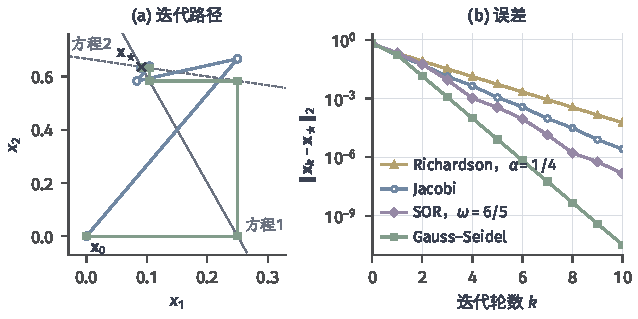
\includegraphics[width=108mm]{figures/01-basic-mathematics/03-vectors-matrices-and-multivariate-functions/matplotlib/c5-stationary-iteration-paths/figure.pdf}
  \caption{定常迭代在贯穿例$\bm A=\begin{bmatrix}4&1\\1&3\end{bmatrix}$，$\bm b=(1,2)^\top$，$\bm x_0=\bm 0$上的真实迭代值。左：实线与虚线分别是第一、第二个方程的解集，两者交于$\bm x_\star=(1/11,7/11)^\top$；蓝色圆点为Jacobi前四轮的迭代点，绿色折线为Gauss--Seidel前三轮的逐坐标路径。右：Richardson（$\alpha=1/4$）、Jacobi、SOR（$\omega=6/5$）与Gauss--Seidel的误差$\lVert\bm x_k-\bm x_\star\rVert_2$，纵轴取对数，渐近斜率分别对应谱半径约$0.40$、$0.29$、$0.20$与$1/12$。}
  \label{fig:ls-stationary-iteration-paths}
\end{figure}

\section{SOR迭代}
\label{sec:ls-sor}

Gauss--Seidel的每个分量修正都恰好让当前方程成立，修正幅度是固定的。\term{逐次超松弛迭代}（successive over-relaxation，SOR）引入固定的\term{松弛参数}（relaxation parameter）$\omega\neq0$，把每个分量的这一修正乘以$\omega$，目的是在误差沿同一方向缓慢衰减时走得更快，或在修正过冲时收敛得更稳。

这相当于把下三角修正矩阵的对角部分除以$\omega$，取$\bm M=\frac1\omega\bm D+\bm L$。$\omega=1$就是Gauss--Seidel；$0<\omega<1$称为欠松弛，只走一部分；$\omega>1$称为过松弛，越过Gauss--Seidel的修正继续走。松弛参数改变的是修正，目标方程没有变。

\paragraph{求修正量}
修正方程$\bigl(\frac1\omega\bm D+\bm L\bigr)\bm\delta_k=\bm r_k$按元素写出是
\[
 \begin{bmatrix}\frac{a_{1,1}}{\omega}&&&\\a_{2,1}&\frac{a_{2,2}}{\omega}&&\\\vdots&\vdots&\ddots&\\a_{d,1}&a_{d,2}&\cdots&\frac{a_{d,d}}{\omega}\end{bmatrix}
 \begin{bmatrix}(\bm\delta_k)_1\\(\bm\delta_k)_2\\\vdots\\(\bm\delta_k)_d\end{bmatrix}
 =\begin{bmatrix}(\bm r_k)_1\\(\bm r_k)_2\\\vdots\\(\bm r_k)_d\end{bmatrix},
\]
其中对角线以上的空白位置都是零。第$i$行的方程是
\[
 \sum_{j<i}a_{i,j}(\bm\delta_k)_j+\frac{a_{i,i}}{\omega}(\bm\delta_k)_i=(\bm r_k)_i\qquad(i=1,\ldots,d).
\]
两边乘以$\omega$，各行合起来就是$(\bm D+\omega\bm L)\bm\delta_k=\omega\bm r_k$，与上面的方程等价。系数矩阵仍是下三角矩阵，按前代求解。第一个方程只含$(\bm\delta_k)_1$，得
\[
 (\bm\delta_k)_1=\frac{\omega(\bm r_k)_1}{a_{1,1}} .
\]
第二个方程中$(\bm\delta_k)_1$已经求出，移项后得
\[
 (\bm\delta_k)_2=\frac{\omega}{a_{2,2}}\bigl((\bm r_k)_2-a_{2,1}(\bm\delta_k)_1\bigr) .
\]
一般地，把第$i$个方程中已经求出的前$i-1$个分量移到右边，再乘以$\omega/a_{i,i}$，得
\begin{equation}
 (\bm\delta_k)_i=\frac{\omega}{a_{i,i}}\Bigl((\bm r_k)_i-\sum_{j<i}a_{i,j}(\bm\delta_k)_j\Bigr)\qquad(i=1,\ldots,d).
 \label{eq:ls-sor-correction}
\end{equation}
括号里仍是前$i-1$个分量修正之后第$i$个方程的残差，除以$a_{i,i}$就是Gauss--Seidel在此刻给出的修正，SOR再把它乘以$\omega$。$\omega=1$时上式逐项退化为式~\eqref{eq:ls-gauss-seidel-correction}。前面的$(\bm\delta_k)_j$已经是松弛后的修正，所以SOR不等于先做一轮Gauss--Seidel再把整个修正量乘以$\omega$。

\paragraph{迭代公式}
把式~\eqref{eq:ls-sor-correction}加到当前近似上，得到第$i$个分量的新值
\begin{equation}
 \begin{aligned}
 (\bm x_{k+1})_i&=(\bm x_k)_i+\frac{\omega}{a_{i,i}}\Bigl((\bm r_k)_i-\sum_{j<i}a_{i,j}(\bm\delta_k)_j\Bigr),\\
 i&=1,\ldots,d,
 \end{aligned}
 \label{eq:ls-sor-update}
\end{equation}
写成向量形式是
\[
 \bm x_{k+1}=\bm x_k+\omega(\bm D+\omega\bm L)^{-1}\bm r_k .
\]

\subsection{算法实现}

输入是$\bm A$与$\bm b$，输出是近似解$\bm x$。除执行流程的参数外，还要预先选定松弛参数$\omega$和变量顺序，顺序固定为$1,\ldots,d$。停止检查与残差重算沿用第~\ref{sec:ls-matrix-splitting}节的流程，求修正量的一步换成带松弛参数的前代；与Gauss--Seidel一样，本轮的$\bm r_k$在整轮中保持不变。下面在例~\ref{ex:ls-stationary-running-example}上取$\omega=6/5$给出前两轮。
\begin{enumerate}
 \item \textbf{核对参数与对角元。}确认所有$a_{i,i}\neq0$。参数是否合格与矩阵是否满足假设是两项不同的检查：对称正定情形的收敛保证（定理~\ref{thm:ls-sor-convergence}）要求$0<\omega<2$，同时要求$\bm A$确实对称正定。

 例中$\bm A$对称正定，$\omega=6/5$在$(0,2)$内。

 \item \textbf{按顺序求修正量。}根据式~\eqref{eq:ls-sor-correction}，对$i=1,\ldots,d$依次计算$(\bm\delta_k)_i$。后面的行扣除的是前面已经松弛后的修正。

 例中第一轮的残差为$\bm r_0=\bm b=(1,2)^\top$：
 \[
  \begin{aligned}
  (\bm\delta_0)_1&=\frac{\omega}{a_{1,1}}(\bm r_0)_1=\frac{6/5}{4}\cdot1=\frac3{10},\\
  (\bm\delta_0)_2&=\frac{\omega}{a_{2,2}}\bigl((\bm r_0)_2-a_{2,1}(\bm\delta_0)_1\bigr)=\frac{6/5}{3}\Bigl(2-1\cdot\tfrac3{10}\Bigr)=\frac{17}{25} .
  \end{aligned}
 \]
 第二行扣除的是松弛后的$3/10$，而不是Gauss--Seidel的$1/4$。

 若先做完整一轮Gauss--Seidel，再把修正量乘以$\omega$，得到的是$\tfrac65(1/4,7/12)^\top=(3/10,7/10)^\top$，与$\bm\delta_0$不同；这一般是另一种方法，不是SOR。

 \item \textbf{更新并重算残差。}根据式~\eqref{eq:ls-sor-update}，令$(\bm x_{k+1})_i=(\bm x_k)_i+(\bm\delta_k)_i$，再按原方程重算残差。与Gauss--Seidel一样，也可以在一个向量上原位逐分量更新，处理第$i$行时现算这一行的残差。

 例中$\bm x_1=\bm x_0+\bm\delta_0=(3/10,17/25)^\top$，
 \[
  \begin{aligned}
  (\bm r_1)_1&=1-\bigl(4\cdot\tfrac3{10}+1\cdot\tfrac{17}{25}\bigr)=1-\tfrac{47}{25}=-\tfrac{22}{25},\\
  (\bm r_1)_2&=2-\bigl(1\cdot\tfrac3{10}+3\cdot\tfrac{17}{25}\bigr)=2-\tfrac{117}{50}=-\tfrac{17}{50} .
  \end{aligned}
 \]
 与第~\ref{sec:ls-gauss-seidel}节不同，第二个方程不再恰好成立，因为它的修正被放大了五分之一。

 \item \textbf{进入下一轮。}令$k\leftarrow k+1$，回到执行流程的停止检查；没有停止时重复第2、3步。

 例中$\lVert\bm r_1\rVert_2\approx0.94$，继续第二轮。用$\bm r_1=(-22/25,-17/50)^\top$求修正量：
 \[
  \begin{aligned}
  (\bm\delta_1)_1&=\frac{6/5}{4}\cdot\Bigl(-\frac{22}{25}\Bigr)=-\frac{33}{125},\\
  (\bm\delta_1)_2&=\frac{6/5}{3}\Bigl(-\frac{17}{50}-1\cdot\Bigl(-\frac{33}{125}\Bigr)\Bigr)\\
  &=\frac25\cdot\Bigl(-\frac{19}{250}\Bigr)=-\frac{19}{625},
  \end{aligned}
 \]
 于是
 \[
  \bm x_2=\bm x_1+\bm\delta_1=\begin{bmatrix}\tfrac3{10}-\tfrac{33}{125}\\\tfrac{17}{25}-\tfrac{19}{625}\end{bmatrix}=\begin{bmatrix}\tfrac9{250}\\\tfrac{406}{625}\end{bmatrix}.
 \]
 重算残差得
 \[
  \begin{aligned}
  (\bm r_2)_1&=1-\bigl(4\cdot\tfrac9{250}+1\cdot\tfrac{406}{625}\bigr)=\tfrac{129}{625},\\
  (\bm r_2)_2&=2-\bigl(1\cdot\tfrac9{250}+3\cdot\tfrac{406}{625}\bigr)=\tfrac{19}{1250} .
  \end{aligned}
 \]
\end{enumerate}

就这个例子而言，过松弛并没有带来好处：两轮的残差长度约为$0.94$与$0.21$，都大于Gauss--Seidel的$0.58$与$0.049$。有限轮的算例只用来解释计算过程；参数的优劣要由下面的谱半径判断。

\subsection{算法分析}

\paragraph{收敛条件}
由迭代公式的向量形式，SOR的修正矩阵满足$\bm M^{-1}=\omega(\bm D+\omega\bm L)^{-1}$，迭代矩阵为
\begin{equation}
\begin{aligned}
\bm T_\omega&=\bm I-\omega(\bm D+\omega\bm L)^{-1}\bm A\\
&=(\bm D+\omega\bm L)^{-1}\bigl[(1-\omega)\bm D-\omega\bm U\bigr],
\end{aligned}
 \label{eq:ls-sor-iteration-matrix}
\end{equation}
第二个等号用到$(\bm D+\omega\bm L)-\omega(\bm D+\bm L+\bm U)=(1-\omega)\bm D-\omega\bm U$。
$\omega$同时影响每个坐标的修正幅度与整轮的误差传播，所以不能随意取：它的取值范围对一般矩阵有一条必要条件，对实对称正定矩阵则恰好也是充分条件。
\begin{theorem}[SOR迭代的收敛条件]
\label{thm:ls-sor-convergence}
设$\bm A$的对角元全不为零。
\begin{enumerate}
\item 对任意这样的方阵，$\rho(\bm T_\omega)\geq|1-\omega|$；所以SOR对所有初值收敛的必要条件是$0<\omega<2$。
\item 若$\bm A$实对称正定且$0<\omega<2$，则$\rho(\bm T_\omega)<1$，SOR对所有初值收敛。
\end{enumerate}
\end{theorem}
\begin{proof}
（1）$\bm D+\omega\bm L$是下三角阵，行列式为$\prod_i a_{i,i}$；$(1-\omega)\bm D-\omega\bm U$是上三角阵，行列式为$(1-\omega)^d\prod_i a_{i,i}$。所以
\[
 \det\bm T_\omega=(1-\omega)^d .
\]
行列式等于全部特征值之积，其模不超过$\rho(\bm T_\omega)^d$，故$\rho(\bm T_\omega)\geq|1-\omega|$。若$\omega\leq0$或$\omega\geq2$，则$\rho(\bm T_\omega)\geq1$，由定理~\ref{thm:ls-stationary-convergence}不能对所有初值收敛。

（2）第$i$次坐标修正的步长是$t=\omega r_i/a_{i,i}$，代入定理~\ref{thm:ls-gauss-seidel-convergence}证明中的能量变化式，$\phi$减少
\[
\omega\frac{r_i^2}{a_{i,i}}-\frac{\omega^2}{2}\frac{r_i^2}{a_{i,i}}=\frac{\omega(2-\omega)\,r_i^2}{2a_{i,i}} .
\]
当$0<\omega<2$时这是非负量，且只在$r_i=0$时为零。此后的论证与该证明相同：一整轮能量不减少只能是$\bm e_k=\bm0$，于是$\bm A-\bm T_\omega^\top\bm A\bm T_\omega$正定，再由特征向量的二次型得$\rho(\bm T_\omega)<1$。
\end{proof}

\paragraph{参数选择与代价}
区间内收敛不等于每个参数都比Gauss--Seidel快。收敛速度取决于参数和变量排列：三对角等特殊结构的矩阵有由$\rho(\bm T_{\mathrm J})$给出的最优参数公式，但不能普遍套用。

贯穿例的$\omega=6/5$就使谱半径从Gauss--Seidel的$1/12$升到$0.2$。$\omega$接近区间端点时，由第一部分$\rho(\bm T_\omega)\geq|1-\omega|$接近一，收敛可能很弱。一轮成本与Gauss--Seidel同阶。

\section{SSOR迭代}
\label{sec:ls-ssor}

单向扫掠依赖变量顺序，对应的$\bm M=\bm D/\omega+\bm L$也不对称。对实对称正定的$\bm A$，\term{对称逐次超松弛迭代}（symmetric SOR，SSOR）把一次前向SOR扫掠与一次反向SOR扫掠配成一轮，参数取固定的$0<\omega<2$。

前向扫掠按$i=1,\ldots,d$的顺序做一次第~\ref{sec:ls-sor}节的SOR，得到中间近似$\bm x_{k+1/2}$；反向扫掠再按$i=d,\ldots,1$的顺序做一次SOR，每个坐标用后面的新值和前面的半步值，得到$\bm x_{k+1}$。

由对称性$\bm U=\bm L^\top$，记$\bm F=\bm D+\omega\bm L$，则$\bm F^\top=\bm D+\omega\bm U$。算法分析将证明，这两次扫掠合起来等价于取修正矩阵
\begin{equation}
 \bm M_{\mathrm{SSOR}}=\frac{1}{\omega(2-\omega)}\bm F\bm D^{-1}\bm F^\top .
 \label{eq:ls-ssor-correction-matrix}
\end{equation}
它是一个下三角、一个对角和一个上三角因子之积，修正方程可以逐个因子求解；它还对称正定，所以SSOR除了单独迭代，还能为第~\ref{chap:krylov-methods}章的共轭梯度法提供预条件。

\paragraph{求修正量}
修正方程$\bm M_{\mathrm{SSOR}}\bm\delta_k=\bm r_k$两边乘以$\omega(2-\omega)$，得
\[
 \bm F\bm D^{-1}\bm F^\top\bm\delta_k=\omega(2-\omega)\bm r_k .
\]
令$\bm z=\bm\delta_k/\bigl(\omega(2-\omega)\bigr)$，$\bm y=\bm D^{-1}\bm F^\top\bm z$，它拆成两个三角方程：先前代解$\bm F\bm y=\bm r_k$，再回代解$\bm F^\top\bm z=\bm D\bm y$，最后$\bm\delta_k=\omega(2-\omega)\bm z$。

下三角因子按元素写出是
\[
 \bm F=\begin{bmatrix}a_{1,1}&&&\\\omega a_{2,1}&a_{2,2}&&\\\vdots&\vdots&\ddots&\\\omega a_{d,1}&\omega a_{d,2}&\cdots&a_{d,d}\end{bmatrix},
\]
对角元取$\bm A$的对角元，严格下三角元乘以$\omega$，对角线以上都是零。$\bm F\bm y=\bm r_k$的第$i$行是
\[
 \omega\sum_{j<i}a_{i,j}y_j+a_{i,i}y_i=(\bm r_k)_i\qquad(i=1,\ldots,d).
\]
第一个方程只含$y_1$，得$y_1=(\bm r_k)_1/a_{1,1}$；此后第$i$个方程中$y_1,\ldots,y_{i-1}$已经求出，移项后除以$a_{i,i}$，得
\begin{equation}
 y_i=\frac{(\bm r_k)_i-\omega\sum_{j<i}a_{i,j}y_j}{a_{i,i}}\qquad(i=1,\ldots,d).
 \label{eq:ls-ssor-forward}
\end{equation}

上三角因子$\bm F^\top$的对角元仍是$a_{i,i}$，由对称性，它在$j>i$处的$(i,j)$元为$\omega a_{j,i}=\omega a_{i,j}$；右端$\bm D\bm y$的第$i$个分量是$a_{i,i}y_i$。所以$\bm F^\top\bm z=\bm D\bm y$的第$i$行是
\[
 a_{i,i}z_i+\omega\sum_{j>i}a_{i,j}z_j=a_{i,i}y_i\qquad(i=1,\ldots,d).
\]
这次最后一个方程只含$z_d$，得$z_d=y_d$；此后第$i$个方程中$z_{i+1},\ldots,z_d$已经求出，移项后除以$a_{i,i}$，得
\begin{equation}
 z_i=y_i-\frac{\omega}{a_{i,i}}\sum_{j>i}a_{i,j}z_j\qquad(i=d,d-1,\ldots,1).
 \label{eq:ls-ssor-backward}
\end{equation}
最后乘以常数，
\begin{equation}
 (\bm\delta_k)_i=\omega(2-\omega)z_i\qquad(i=1,\ldots,d).
 \label{eq:ls-ssor-correction}
\end{equation}

\paragraph{迭代公式}
把式~\eqref{eq:ls-ssor-correction}加到当前近似上，得到第$i$个分量的新值
\begin{equation}
 (\bm x_{k+1})_i=(\bm x_k)_i+\omega(2-\omega)z_i\qquad(i=1,\ldots,d),
 \label{eq:ls-ssor-update}
\end{equation}
其中$\bm z$由式~\eqref{eq:ls-ssor-forward}与式~\eqref{eq:ls-ssor-backward}依次求出。写成向量形式是
\[
 \bm x_{k+1}=\bm x_k+\omega(2-\omega)\bm F^{-\top}\bm D\bm F^{-1}\bm r_k .
\]

\subsection{算法实现}

输入是实对称正定的$\bm A$与$\bm b$，输出是近似解$\bm x$。除执行流程的参数外，还要预先选定$\omega$。停止检查与残差重算沿用第~\ref{sec:ls-matrix-splitting}节的流程，求修正量的一步换成一次前代与一次回代，内部多两个与$\bm x$同长的向量$\bm y$与$\bm z$。下面在例~\ref{ex:ls-stationary-running-example}上取$\omega=1$给出前两轮；这时$\bm F=\bm D+\bm L=\left[\begin{smallmatrix}4&0\\1&3\end{smallmatrix}\right]$，$\omega(2-\omega)=1$。
\begin{enumerate}
 \item \textbf{核对条件。}确认$\bm A$对称正定且$0<\omega<2$；正定矩阵的对角元都为正，所以各次除法都能执行。

 例中$\bm A$对称正定，$a_{1,1}=4$，$a_{2,2}=3$，$\omega=1$。

 \item \textbf{前代。}根据式~\eqref{eq:ls-ssor-forward}，对$i=1,\ldots,d$依次计算$y_i$，右端是本轮开始时的残差$\bm r_k$。

 例中第一轮的残差为$\bm r_0=\bm b=(1,2)^\top$：
 \[
  \begin{aligned}
  y_1&=\frac{(\bm r_0)_1}{a_{1,1}}=\frac14,\\
  y_2&=\frac{(\bm r_0)_2-\omega a_{2,1}y_1}{a_{2,2}}=\frac{2-1\cdot\tfrac14}{3}=\frac7{12} .
  \end{aligned}
 \]
 $\omega=1$时$\bm F=\bm D+\bm L$，$\bm y$就是Gauss--Seidel的修正量$\bm\delta_0$。

 \item \textbf{回代并缩放。}根据式~\eqref{eq:ls-ssor-backward}，对$i=d,\ldots,1$依次计算$z_i$，再按式~\eqref{eq:ls-ssor-correction}乘以$\omega(2-\omega)$得到$\bm\delta_k$。

 例中先处理第二行，再用刚得到的$z_2$处理第一行：
 \[
  \begin{aligned}
  z_2&=y_2=\frac7{12},\\
  z_1&=y_1-\frac{\omega}{a_{1,1}}a_{1,2}z_2=\frac14-\frac14\cdot\frac7{12}=\frac5{48},
  \end{aligned}
 \]
 所以$\bm\delta_0=\bm z=(5/48,7/12)^\top$。

 \item \textbf{更新并重算残差。}根据式~\eqref{eq:ls-ssor-update}，令$(\bm x_{k+1})_i=(\bm x_k)_i+(\bm\delta_k)_i$，再按原方程重算$\bm r_{k+1}=\bm b-\bm A\bm x_{k+1}$。

 例中$\bm x_1=\bm x_0+\bm\delta_0=(5/48,7/12)^\top$，
 \[
  \begin{aligned}
  (\bm r_1)_1&=1-\bigl(4\cdot\tfrac5{48}+1\cdot\tfrac7{12}\bigr)=0,\\
  (\bm r_1)_2&=2-\bigl(1\cdot\tfrac5{48}+3\cdot\tfrac7{12}\bigr)=\tfrac7{48} .
  \end{aligned}
 \]
 这次为零的是第一个分量，因为按双向扫掠来看，反向扫掠最后修正的是第一行。

 \item \textbf{进入下一轮。}令$k\leftarrow k+1$，回到执行流程的停止检查；没有停止时重复第2至4步。

 例中$\lVert\bm r_1\rVert_2=7/48\approx0.15$，继续第二轮。由$\bm r_1=(0,7/48)^\top$，前代与回代给出
 \[
  \begin{aligned}
  y_1&=\frac{0}{4}=0, & y_2&=\frac{\tfrac7{48}-1\cdot0}{3}=\frac7{144},\\
  z_2&=y_2=\frac7{144}, & z_1&=0-\frac14\cdot\frac7{144}=-\frac7{576},
  \end{aligned}
 \]
 于是
 \[
  \bm x_2=\bm x_1+\bm z=\begin{bmatrix}\tfrac5{48}-\tfrac7{576}\\\tfrac7{12}+\tfrac7{144}\end{bmatrix}=\begin{bmatrix}\tfrac{53}{576}\\\tfrac{91}{144}\end{bmatrix}.
 \]
 重算残差得
 \[
  \begin{aligned}
  (\bm r_2)_1&=1-\bigl(4\cdot\tfrac{53}{576}+1\cdot\tfrac{91}{144}\bigr)=0,\\
  (\bm r_2)_2&=2-\bigl(1\cdot\tfrac{53}{576}+3\cdot\tfrac{91}{144}\bigr)=\tfrac7{576} .
  \end{aligned}
 \]
 两轮中各个三角子问题都精确解出了，残差却仍不为零。验收用的是原方程的残差，不能以子问题已经解完代替。
\end{enumerate}

\paragraph{双向扫掠}
等价的实现按本节开头的描述做两次SOR扫掠，代替上面的第2、3步。前向扫掠按式~\eqref{eq:ls-sor-correction}由$\bm r_k$求出修正量$\bm\delta_{\mathrm f}$，令$\bm x_{k+1/2}=\bm x_k+\bm\delta_{\mathrm f}$，再按原方程算出半步后的残差$\bm r_{k+1/2}=\bm b-\bm A\bm x_{k+1/2}$。

反向扫掠按$i=d,\ldots,1$的顺序求
\begin{equation}
 (\bm\delta_{\mathrm b})_i=\frac{\omega}{a_{i,i}}\Bigl((\bm r_{k+1/2})_i-\sum_{j>i}a_{i,j}(\bm\delta_{\mathrm b})_j\Bigr),
 \label{eq:ls-ssor-backward-sweep}
\end{equation}
令$\bm x_{k+1}=\bm x_{k+1/2}+\bm\delta_{\mathrm b}$。反向扫掠的右端必须是半步后的残差，不能继续使用本轮开始时的$\bm r_k$。

两次扫掠也都可以在同一个向量上原位逐坐标更新，每行的残差在访问时现算，不必单独形成$\bm r_{k+1/2}$。算法分析中的推导说明，两次修正之和正是式~\eqref{eq:ls-ssor-correction}给出的$\bm\delta_k$。

例中第一轮的前向扫掠就是一轮Gauss--Seidel，给出
\[
 \bm\delta_{\mathrm f}=\bm x_{1/2}=\begin{bmatrix}1/4\\7/12\end{bmatrix},\qquad
 \bm r_{1/2}=\begin{bmatrix}-7/12\\0\end{bmatrix}.
\]
反向扫掠先处理第二行，再处理第一行：
\[
 (\bm\delta_{\mathrm b})_2=\frac{0}{3}=0,\qquad
 (\bm\delta_{\mathrm b})_1=\frac{-\tfrac7{12}-1\cdot0}{4}=-\frac7{48},
\]
所以$\bm x_1=(1/4-7/48,\,7/12)^\top=(5/48,7/12)^\top$，与因子求解一致。第二分量保持不变，因为前向扫掠的最后一步已经让第二个方程成立。

\paragraph{作为预条件}
作为共轭梯度法的预条件使用时，SSOR不更新近似解，只把外层迭代给出的残差$\bm r$变成修正方向：以$\bm r$代替$\bm r_k$，按式~\eqref{eq:ls-ssor-forward}、式~\eqref{eq:ls-ssor-backward}前代、回代并缩放，返回$\bm M_{\mathrm{SSOR}}^{-1}\bm r$，近似解由外层方法另行更新。同一次外层求解中，$\omega$和三角因子要保持不变，否则预条件矩阵逐轮变化，外层方法依赖的固定内积结构就不成立。具体用法见第~\ref{sec:ls-preconditioning}节。

\subsection{算法分析}

\paragraph{修正矩阵}
先把两次扫掠的修正合并成一个修正矩阵，并确定缩放常数，使独立迭代与作为预条件的实现使用同一约定。

前向半步就是一次SOR：解$\bm F\bm\delta_{\mathrm f}=\omega\bm r_k$，令$\bm x_{k+1/2}=\bm x_k+\bm\delta_{\mathrm f}$。

反向半步按$i=d,\ldots,1$的顺序做SOR，先访问的是下标大的分量，所以本轮新值出现在上三角部分，对应的方程是$\bm F^\top\bm\delta_{\mathrm b}=\omega\bm r_{k+1/2}$，再令$\bm x_{k+1}=\bm x_{k+1/2}+\bm\delta_{\mathrm b}$。右端是半步后的残差
\[
\bm r_{k+1/2}=\bm b-\bm A\bm x_{k+1/2}=\bm r_k-\bm A\bm\delta_{\mathrm f}.
\]

把两次修正相加。由$\bm\delta_{\mathrm f}=\omega\bm F^{-1}\bm r_k$，
\[
\begin{aligned}
\bm\delta_{\mathrm f}+\bm\delta_{\mathrm b}
&=\omega\bm F^{-1}\bm r_k+\omega\bm F^{-\top}\bigl(\bm r_k-\omega\bm A\bm F^{-1}\bm r_k\bigr)\\
&=\omega\bm F^{-\top}\bigl(\bm F^\top\bm F^{-1}+\bm F\bm F^{-1}-\omega\bm A\bm F^{-1}\bigr)\bm r_k\\
&=\omega\bm F^{-\top}\bigl(\bm F^\top+\bm F-\omega\bm A\bigr)\bm F^{-1}\bm r_k ,
\end{aligned}
\]
第二个等号在第一项前插入$\bm F^{-\top}\bm F^\top$，在第二项中插入$\bm F\bm F^{-1}$。又由$\bm F=\bm D+\omega\bm L$与$\bm F^\top=\bm D+\omega\bm U$，
\[
\begin{aligned}
\bm F^\top+\bm F-\omega\bm A
&=2\bm D+\omega(\bm L+\bm U)-\omega(\bm D+\bm L+\bm U)\\
&=(2-\omega)\bm D ,
\end{aligned}
\]
所以一整轮的修正为
\begin{equation}
\bm\delta_k=\omega(2-\omega)\,\bm F^{-\top}\bm D\bm F^{-1}\bm r_k ,
 \label{eq:ls-ssor-combined-correction}
\end{equation}
即$\bm M_{\mathrm{SSOR}}\bm\delta_k=\bm r_k$，$\bm M_{\mathrm{SSOR}}$就是本节开头给出的矩阵。

求解的次序是先解$\bm F$、再乘$\bm D$、最后解$\bm F^\top$，不必显式形成$\bm M_{\mathrm{SSOR}}$或它的逆；算法实现的第2、3步正是按这个次序。

这个修正矩阵对称正定。对称性由形式$\bm F\bm D^{-1}\bm F^\top$直接看出。$\bm A$正定，把第$i$个坐标单位向量代入二次型即得$a_{i,i}>0$，所以$\bm D\succ0$；$\bm F$是对角元为正的下三角阵，可逆。于是对$\bm v\neq\bm0$，
\[
\bm v^\top\bm M_{\mathrm{SSOR}}\bm v=\frac{(\bm F^\top\bm v)^\top\bm D^{-1}(\bm F^\top\bm v)}{\omega(2-\omega)}>0 ,
\]
这里用到$0<\omega<2$使分母为正。注意对称正定的是修正矩阵$\bm M_{\mathrm{SSOR}}$；迭代矩阵$\bm I-\bm M_{\mathrm{SSOR}}^{-1}\bm A$一般不是对称矩阵。

\paragraph{收敛性}
$\bm M_{\mathrm{SSOR}}$正定本身还不足以断言定常迭代收敛；还需要它在二次型意义下不小于$\bm A$。先展开
\[
 \bm F\bm D^{-1}\bm F^\top=\bm D+\omega\bm L+\omega\bm U+\omega^2\bm L\bm D^{-1}\bm U ,
\]
再减去$\omega(2-\omega)\bm A=\omega(2-\omega)(\bm D+\bm L+\bm U)$，整理得
\[
\begin{aligned}
\omega(2-\omega)(\bm M_{\mathrm{SSOR}}-\bm A)
&=(1-\omega)^2\bm D-\omega(1-\omega)(\bm L+\bm U)+\omega^2\bm L\bm D^{-1}\bm U\\
&=\bm C\bm D^{-1}\bm C^\top ,
\end{aligned}
\]
其中$\bm C=(1-\omega)\bm D-\omega\bm L$，最后一步把$\bm C\bm D^{-1}\bm C^\top$展开即可核对。因为$\bm D\succ0$，$\bm C\bm D^{-1}\bm C^\top\succeq0$，所以
\begin{equation}
\bm 0\prec\bm A\preceq\bm M_{\mathrm{SSOR}} .
 \label{eq:ls-ssor-dominates}
\end{equation}

由此读出迭代矩阵的谱。$\bm M_{\mathrm{SSOR}}$对称正定，有正定平方根（第~\ref{sec:ls-matrix-square-root}节）。令$\bm S=\bm M_{\mathrm{SSOR}}^{-1/2}\bm A\bm M_{\mathrm{SSOR}}^{-1/2}$，它实对称。若$\bm S\bm w=\mu\bm w$，$\bm w\neq\bm0$，令$\bm y=\bm M_{\mathrm{SSOR}}^{-1/2}\bm w$，则
\[
\mu=\frac{\bm w^\top\bm S\bm w}{\bm w^\top\bm w}=\frac{\bm y^\top\bm A\bm y}{\bm y^\top\bm M_{\mathrm{SSOR}}\bm y}\in(0,1].
\]
迭代矩阵可以写成
\[
 \bm T_{\mathrm{SSOR}}=\bm I-\bm M_{\mathrm{SSOR}}^{-1}\bm A=\bm M_{\mathrm{SSOR}}^{-1/2}(\bm I-\bm S)\bm M_{\mathrm{SSOR}}^{1/2} ,
\]
它与实对称矩阵$\bm I-\bm S$相似，特征值$1-\mu$全部落在$[0,1)$中，所以$\rho(\bm T_{\mathrm{SSOR}})<1$。

由定理~\ref{thm:ls-stationary-convergence}，在$\bm A$实对称正定、$0<\omega<2$时SSOR对所有初值收敛。这里$\bm T_{\mathrm{SSOR}}$本身一般不对称，只是相似于对称矩阵，因而特征值为实数。

\paragraph{代价与用途}
一轮含两次三角扫掠（或等价的前代、对角缩放与回代），另加一次计算残差的矩阵乘向量，工作量约为SOR一轮的两倍；存储只多一个与$\bm x$同长的中间向量。

比较时不能只数轮数：贯穿例中$\omega=1$的SSOR谱半径为$1/12$，与Gauss--Seidel相同，每轮却多花一倍计算。SSOR作为独立迭代往往并不比SOR省；它的主要价值在于对称正定的修正矩阵：作为预条件时，每次外层迭代多付两次三角求解，换来外层共轭梯度法所需步数的减少，是否划算要按总成本比较（第~\ref{sec:ls-preconditioning}节）。

\section{收敛检验与停止准则}
\label{sec:ls-stationary-stopping}

各方法都使用第~\ref{sec:ls-matrix-splitting}节的终止条件：$\lVert\bm r_k\rVert_2\leq\mathrm{atol}+\mathrm{rtol}\lVert\bm b\rVert_2$，或$k=K$。前者表示达到了给定的残差要求；后者只表示不再继续计算，结果未必达到精度。两种情况下输出都只是当前的$\bm x_k$，所以结束状态必须一并报告。残差用真实的$\bm b-\bm A\bm x_k$计算，而不是只依赖递推值。

几种量不能代替原方程的残差检验。修正量$\lVert\bm\delta_k\rVert$很小，可能只说明收缩因子接近一、迭代走得很慢，而不是已经接近解。残差在很多轮内几乎不降，应作为停滞报告，而不是当作收敛。计算中出现溢出或非数，应作为数值异常报告；这通常说明迭代发散或对角元过小。

残差小也不等于解的误差小。由$\bm x_\star-\bm x_k=\bm A^{-1}\bm r_k$，误差是残差经$\bm A^{-1}$放大的结果，两者之间隔着问题本身的敏感性；第~\ref{sec:ls-numerical-sensitivity}节再给出误差界和后向误差的解释。

比较不同方法时，应在相同精度要求下比较总工作量，而不是轮数；分析中的收敛率和代价用于解释算法，不加入求解器的输出。其他用递推方式维护残差的方法，递推值会因舍入而偏离真实残差，停止前也须用$\bm b-\bm A\bm x_k$复核。

\FloatBarrier
\section{本章小结}
\label{sec:stationary-iterations-summary}

本章回答了怎样不分解$\bm A$而逐步求解可逆方程$\bm A\bm x=\bm b$。共同的做法是矩阵分裂$\bm A=\bm M-\bm N$：每轮解一个以易解矩阵$\bm M$为系数的修正方程$\bm M\bm\delta_k=\bm r_k$，再更新近似解。误差满足$\bm e_{k+1}=(\bm I-\bm M^{-1}\bm A)\bm e_k$，由第~\ref{chap:linear-recurrence-stability}章的矩阵幂结论，迭代对任意初值收敛当且仅当迭代矩阵的谱半径小于一，渐近速度也由谱半径决定。

五种方法的区别只在于$\bm M$怎样近似$\bm A$、数据怎样读取。Richardson取$\bm M=\alpha^{-1}\bm I$，只需矩阵乘向量；对称正定时收敛当且仅当$0<\alpha<2/\lambda_{\max}$，最优步长的收缩因子为$(\kappa_2-1)/(\kappa_2+1)$。Jacobi取$\bm M=\bm D$，各分量只读旧值、可以并行，严格行对角占优保证收敛，对称正定本身不保证。

Gauss--Seidel取$\bm M=\bm D+\bm L$，立即使用本轮新值，相当于一次前代；严格行对角占优或对称正定都保证收敛。SOR取$\bm M=\bm D/\omega+\bm L$，$0<\omega<2$对一般矩阵是必要条件，对对称正定矩阵也是充分条件；区间内不同参数的速度仍须比较。SSOR把前向与反向SOR配成一轮，修正矩阵$\bm M_{\mathrm{SSOR}}=\bm F\bm D^{-1}\bm F^\top/[\omega(2-\omega)]$对称正定且满足$\bm A\preceq\bm M_{\mathrm{SSOR}}$，由此证明收敛，并可作为共轭梯度法的预条件。

这些结论都有边界。对角元非零只保证可执行，不保证收敛；用了新信息、加了过松弛，都不自动更快；贯穿例中Gauss--Seidel的谱半径为$1/12$，$\omega=6/5$的SOR反而是$0.2$。比较方法要把谱半径决定的轮数与每轮成本合起来，看达到相同精度的总工作量。

停止计算也要分清含义。只有真实残差满足$\lVert\bm r_k\rVert_2\leq\mathrm{atol}+\mathrm{rtol}\lVert\bm b\rVert_2$才算达到残差目标；步数耗尽、停滞或数值异常都只是停止，修正量很小也不代表接近解。即使残差达标，前向误差仍受问题条件数制约，这在第~\ref{sec:ls-numerical-sensitivity}节讨论；第~\ref{chap:krylov-methods}章则在逐步扩大的子空间中选择近似，以改善定常迭代受谱半径限制的收敛速度。
